\documentclass[%
fontsize=10%
,a5paper%
,DIV=15%
]{scrartcl}
%scrartcl



\usepackage{gredocument}
\usepackage{psaume}

\title{\centrer{Messe de Mariage}}
\author{Avec l'échange des consentements  et la bénédiction nuptiale}
\date{}

\makeindex
\definecolor{rubrum}{rgb}{.6,0,0}
\def\rubrum{\color{rubrum}}%%%%%%%mettre"\def\rubrum{\color{rubrum}}" pour avoir le texte adéquat en rouge
\def\nigra{\color{black}}
%    \redlines
%    \definecolor{gregoriocolor}{rgb}{.6,0,0}
%
%\let\red\rubrum

\begin{document}
    \newfontfamily\lettrines[Scale=1.3]{LettrinesPro800}
    \def\gretextformat#1{{\fontsize{\taillepolice}{\taillepolice}\selectfont #1}}
    \def\greinitialformat#1{{\lettrines #1}}

\titre{Veni Creator}
\vspace{0.5cm}
\rubrica{On se met à genoux pour la première strophe.}
\vulgo{1. Venez, Esprit-Saint Créateur, dans les âmes de vos fidèles : comblez de la grâce d'en haut les c\oe urs que vous avez créés.}

\cantus{Hymne}{VeniCreator}{}{}
\noindent
\traduire{%
2.~Qui díceris Paráclitus,\\%
Altíssimi donum Dei,\\%
Fons vivus, ignis, cáritas\\%
Et spiritális únctio.}{%
2.~Vous qu'on appelle Consolateur,\\%
don du Dieu très-haut,\\%
source vive, feu, charité\\%
et onction spirituelle.\\%

}

\traduire{%
3.~Tu septifórmis múnere,\\%
Dig\textit{i}tus patérnæ déxteræ,\\%
Tu rite promíssum Patris,\\%
Sérmone ditans gúttura.}{%
3.~Vous l'Esprit aux sept dons,\\%
le doigt de Dieu,\\%
la promesse authentique du Père,\\%
qui mettez sa parole sur nos lèvres.\\%

}


\traduire{%
4.~Accénde lumen sénsibus,\\%
Infúnd\textit{e} amórem córdibus,\\%
Infírma nostri córporis\\%
Vírtute firmans pérpeti.}{%
4.~Éclairez nos esprits de votre lumière,\\%
mettez l'amour dans nos c\oe urs~;\\%
soutenez la faiblesse de notre corps\\%
par votre constante vigueur.\\%

}


\traduire{%
5.~Hostem repéllas lóngius,\\%
Pacémque dones prótinus~:\\%
Ductóre sic te pr\'ævio\\%
Vitémus omne nóxium.\\}{%
5.~Chassez l'ennemi loin de nous,\\%
donnez-nous sans retard la paix~;\\%
guidez-nous, et que sous votre conduite\\%
nous évitions tout mal.\\%
}

\traduire{%
6.~Per te sciámus da Patrem,\\%
Noscámus atque Fílium,\\%
Tequ\textit{e} utriúsque Spíritum\\%
Credámus omni témpore.\\}{%
6.~Faites-nous connaître le Père,\\%
faites-nous connaître le Fils,\\%
donnez-nous de toujours croire en vous\\%
qui êtes l'Esprit du Père et du Fils.\\%
}

\traduire{%
7.~Deo Patri sit glória,\\%
Et Fílio qu\textit{i} a mórtuis\\%
Surréxit, ac Paráclito,\\%
In sæculórum sǽcula.\\%
Amen\\}{%
7.~Gloire soit à Dieu le Père,\\%
et au Fils ressuscité des morts,\\%
et à l'Esprit consolateur\\%
dans les siècles des siècles.\\%
\ainsi\\%
}

\traduire{%
℣.~Emitte Spiritum tuum et creabúntur.}{%
℣.~Envoyez votre Esprit Seigneur et il se fera une création nouvelle.}

\traduire{\textbf{%
℟.~Et renovábis fáciem terræ.}}{\textbf{%
℟.~Et vous renouvellerez la face de la terre.}}

\traduire{%
Orémus.}{%
Prions.}

\traduire{%
Deus, qui corda fidélium Sancti Spíritus illustratióne docuísti : da nobis in eódem Spíritu recta sápere, et de eius consolatióne gaudére. \Perdominum \quitecum \peromnia%
}{%
Ô Dieu, qui avez éclairé les cœurs de vos fidèles par la lumière du Saint-Esprit, donnez-nous par ce même Esprit de comprendre et d'aimer ce qui est bien, et de jouir sans cesse de ses divines consolations. \Parjesus \quietant \siecles}
\amen


\titre{Les consentements}

\rubrica{Le prêtre s'adresse au fiancé :}

  \textsc{Mon{s}{i}eur {\rubrum{N.}}, voulez-vous prendre pour légitime épouse {\rubrum{N.}}, ici présente, selon le rite de notre mère la Sainte Eglise?}

\rubrique{Le fiancé répond : }  \textsc{Oui, je le veux.}

\rubrique{Puis, s'adressant à la fiancée :}

  \textsc{Mademoiselle {\rubrum{N.}}, voulez-vous prendre pour légitime époux {\rubrum{N.}}, ici présent, selon le rite de notre mère la Sainte Eglise?}

\rubrique{La fiancée répond : }  \textsc{Oui, je le veux.}

\rubrique{Le prêtre invite alors les époux à se donner la main droite. Puis il confirme l'engagement dont il vient d'être témoin en disant :}

\traduire{Ego conjungo vos in matrimonium, in nomine Patri, et Filii~\x\ et Spiritui Sancti. Amen.}{Je vous déclare unis par le mariage au nom du Père et du Fils~\x\ et du Saint Esprit. Ainsi soit-il.}

\vspace{0.5cm}
\titre{Bénédiction des Anneaux}

\rubrique{Le prêtre bénit les anneaux :}

\traduire{\V Adiutorium nostrum in nomine Domini.}{\V Notre secours est dans le nom du Seigneur.}

\traduire{\R \textbf{Qui fecit c\ae lum et terram.}}{\R \textbf{Qui a fait le ciel et la terre.}}


\traduire{%
\V~Dómine, exáudi oratiónem meam.}{%
\V~Seigneur, exaucez ma prière.}

\traduire{%
\R~\textbf{Et clamor meus ad te véniat.}}{%
\R~\textbf{Que mon appel vous parvienne.}}

\traduire{%
\V~Dóminus vobíscum.}{%
\V~Le Seigneur soit avec vous.}

\traduire{%
\R~\textbf{Et cum spíritu tuo.}}{%
\R~\textbf{Et avec votre esprit.}}

\traduire{%
Orémus.}{%
Prions.}

\traduire{ Bene~\x\ dic Domine annulum hunc quem nos in tuo nomine bene~\x\ dicimus, ut quæ eum gestaverit, fidelitatem integram suo sponso tenens, in pace et voluntate tua permaneat, atque in mutua caritate semper vivat.}{Béni~\x\ ssez, Seigneur, ces anneaux que nous béni~\x\ ssons en votre nom, afin que ceux qui les porteront, les conservent dans une fidélité entière, demeurent dans la paix et dans votre volonté, et qu'ils vivent toujours dans une mutuelle affection. Par le Christ Notre-Seigneur.}

\Amen

\rubrique{L'époux passe au doigt de son épouse et à son doigt l'anneau qui ne les quittera plus.
Le prêtre bénit ce geste et appelle les grâces divines sur l'union irrévocable qui vient de se conclure.}

\titre{Prière pour les époux}

\vspace*{0.5cm}
Au nom du Père~\x\ et du Fils et du Saint-Esprit. Ainsi soit-il.

\V Confirmez, Seigneur, ce que vous avez accompli en nous.

\R \textbf{De votre saint temple, en Jérusalem.}

Seigneur, ayez pitié de nous.
Christ, ayez pitié de nous.
Seigneur, ayez pitié de nous.

Notre Père... (à voix basse)

\V Et ne nous laissez pas succomber à la tentation. 

\R \textbf{Mais délivrez-nous du mal.}

\V Seigneur, sauvez vos serviteurs.

\R \textbf{Qui espèrent en vous, mon Dieu.}

\V Envoyez-leur votre aide, Seigneur, de votre sanctuaire.

\R\textbf{ Et de Sion, soutenez-les.}

\V Soyez pour eux, Seigneur, comme une tour fortifiée.

\R \textbf{Dressée contre l'ennemi.}

\V Seigneur, exaucez ma prière.

\R \textbf{Et que mon appel monte jusqu'à vous.}

\V Le Seigneur soit avec vous.

\R \textbf{Et avec votre esprit.}

Prions\\
Jetez les yeux, Seigneur, sur ces époux vos serviteurs et protégez cette institution que vous avez établie pour la propagation du genre humain, afin qu'unis par vous ils soient également soutenus et gardés par votre secours. Par le Christ Notre-Seigneur.

\R \textbf{Ainsi soit-il.}
\vspace*{3cm}
%\begin{center}
%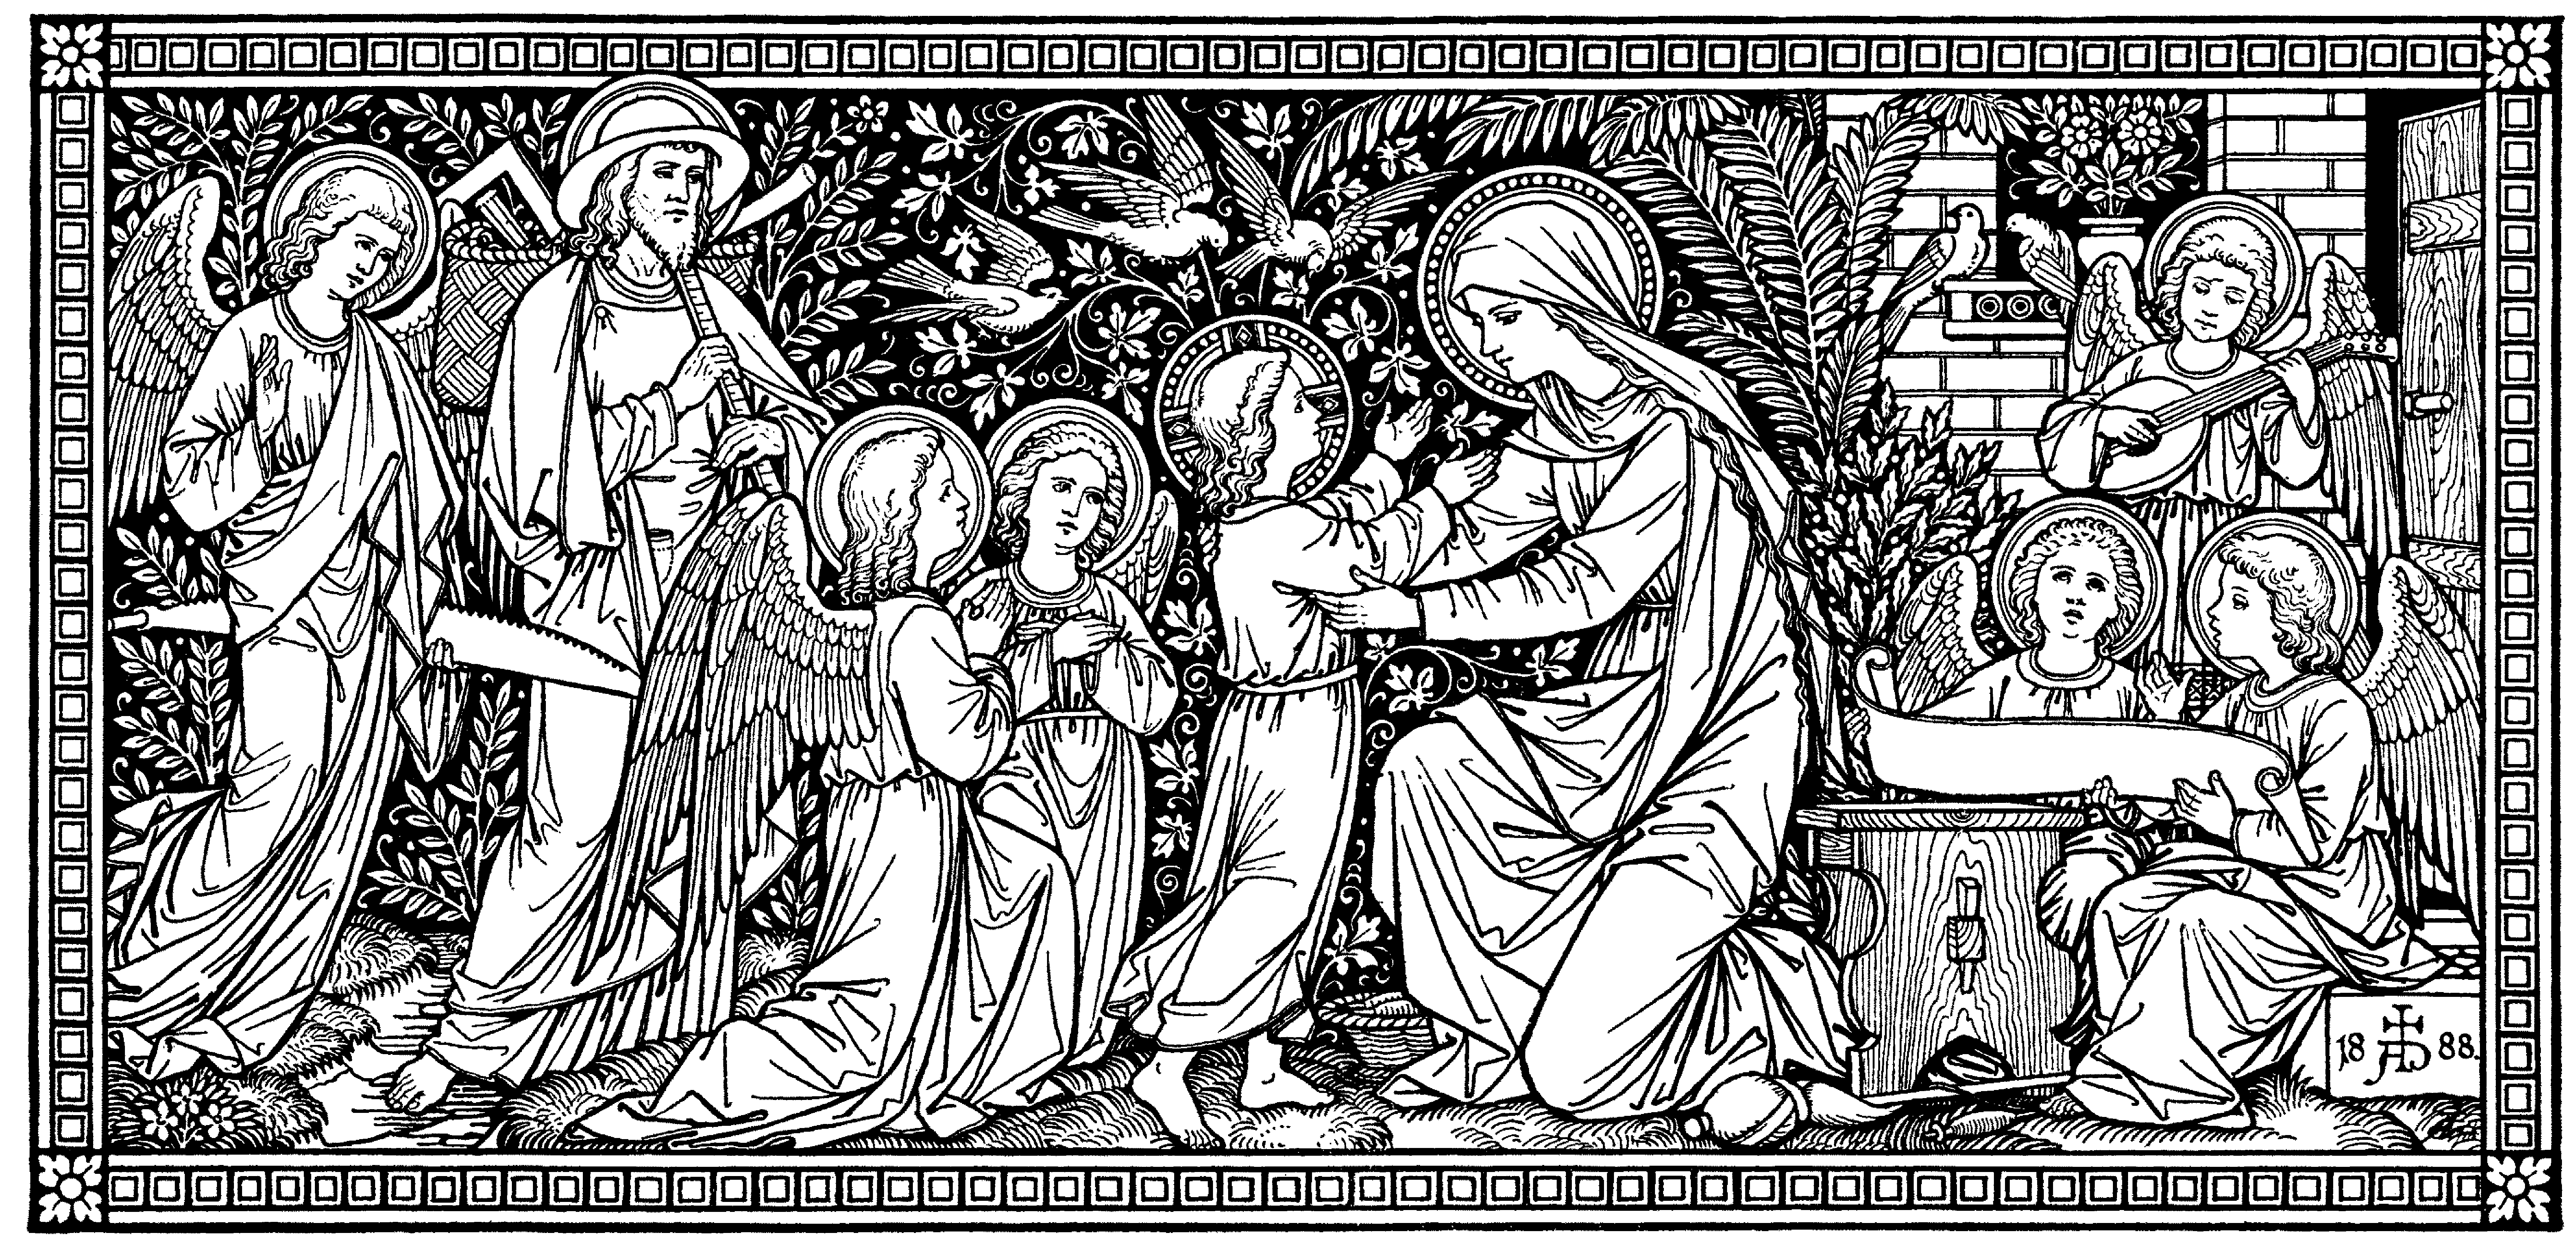
\includegraphics[height=5.5cm]{images/SainteFamille}
%\end{center}





\end{document}